\documentclass{standalone}
%-----------------------------------------------------------------------------%
%%% Color %%%
\usepackage{xcolor}
\definecolor{myred}{RGB}{229,0,0}
\definecolor{myblue}{RGB}{0,98,144}
\definecolor{myyellow}{RGB}{246,182,50}
\newcommand{\red}[1]{\textcolor{myred}{#1}}
\newcommand{\blue}[1]{\textcolor{myblue}{#1}}
\newcommand{\yellow}[1]{\textcolor{myyellow}{#1}}
%-----------------------------------------------------------------------------%
%%% TikZ %%%
\usepackage{tikz}
\usetikzlibrary{calc}
% \usetikzlibrary{positioning}
% \usetikzlibrary{patterns}
% \usetikzlibrary{fit}
\usetikzlibrary{angles,quotes}
% \usetikzlibrary{intersections}
% \usetikzlibrary{decorations.markings}
%-----------------------------------------------------------------------------%
%%% TikZ: Mark Angles %%%
\newcommand{\MarkRightAngle}[5][]{
\draw[#1] let
\p1=($(#3)-(#4)$),\n1={atan2(\y1,\x1)},
\p2=($(#5)-(#4)$),\n2={atan2(\y2,\x2)} in
(#4) -- ++(\n1:#2) -- ++(\n2:#2) -- ++({\n1+180}:#2) --cycle;}
%-----------------------------------------------------------------------------%
\newcommand{\MarkAngle}[5]["$\theta$",->,draw=blue!80,fill=blue!20]{
\pic[#1,angle radius=#2] {angle = #3--#4--#5};}
%-----------------------------------------------------------------------------%
% \MarkAngle     [fill=blue]{0.2cm}{A}{O}{B}{node[pos=0.5]{}}
% \MarkRightAngle[fill=blue]{0.2cm}{A}{O}{B}
%-----------------------------------------------------------------------------%

\begin{document}

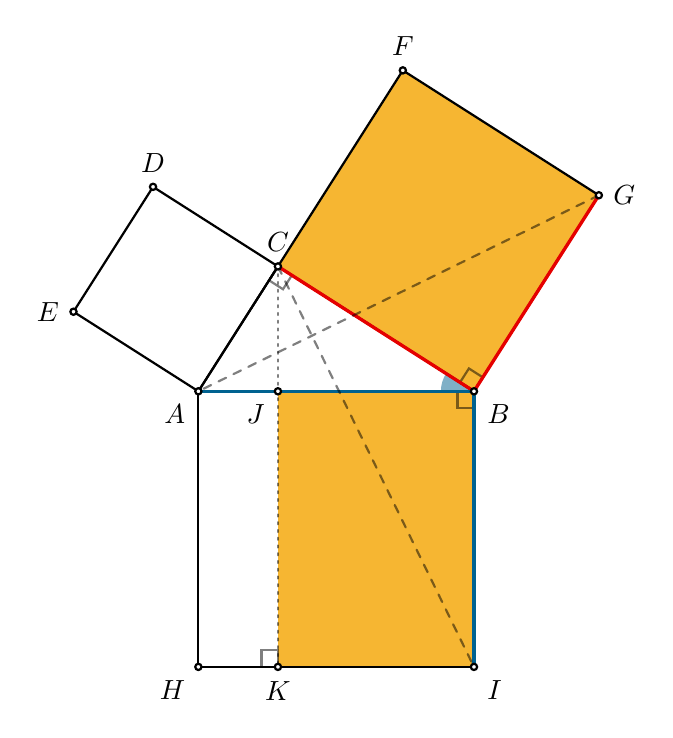
\begin{tikzpicture}[thick,line cap=round]
	\tikzstyle{bai}=[solid,circle,draw,inner sep=.8pt,fill=white];
	\tikzstyle{hei}=[solid,circle,draw,inner sep=.8pt,fill];
	\newcommand{\length}{3.5cm}
	%%
	\coordinate (A) at (0,0);
	\coordinate (B) at (\length,0);
	\coordinate (C) at ($(\length/2,0)+(115:\length/2)$);
	\coordinate (D) at ($(C)!1!-90:(A)$);
	\coordinate (E) at ($(A)!1! 90:(C)$);
	\coordinate (F) at ($(C)!1! 90:(B)$);
	\coordinate (G) at ($(B)!1!-90:(C)$);
	\coordinate (H) at ($(A)+(0,-\length)$);
	\coordinate (I) at ($(B)+(0,-\length)$);
	\path let \p1=(C) in (\x1,0)        -- (\x1,0)        coordinate (J);
	\path let \p1=(J) in (\x1,-\length) -- (\x1,-\length) coordinate (K);
	%%
	\path[fill=myyellow] (B) -- (G) -- (F) -- (C) --cycle;
	\path[fill=myyellow] (J) -- (K) -- (I) -- (B) --cycle;
	%%
	\MarkAngle[fill=myblue,opacity=0.5]{0.12*\length}CBA
	\MarkRightAngle[draw=black,opacity=0.5]{0.06*\length}ACB
	\MarkRightAngle[draw=black,opacity=0.5]{0.06*\length}GBC
	\MarkRightAngle[draw=black,opacity=0.5]{0.06*\length}JBI
	\MarkRightAngle[draw=black,opacity=0.5]{0.06*\length}CKH
	%%
	\draw (A) -- (B) -- (C) --cycle;
	\draw (A) -- (C) -- (D) -- (E) --cycle;
	\draw (B) -- (G) -- (F) -- (C) --cycle;
	\draw (A) -- (H) -- (I) -- (B) --cycle;
	%%
	\draw[very thick,myred] (B) -- (G);
	\draw[very thick,myred] (B) -- (C);
	\draw[very thick,myblue] (B) -- (A);
	\draw[very thick,myblue] (B) -- (I);
	%%
	\draw[draw=black,dotted,opacity=0.5] (C) -- (K);
	\draw[draw=black,dashed,opacity=0.5] (G) -- (A);
	\draw[draw=black,dashed,opacity=0.5] (C) -- (I);
	%%
	\node[bai,label=below left:  {$A$}] at (A) {};
	\node[bai,label=below right: {$B$}] at (B) {};
	\node[bai,label=above:       {$C$}] at (C) {};
	\node[bai,label=above:       {$D$}] at (D) {};
	\node[bai,label=left:        {$E$}] at (E) {};
	\node[bai,label=above:       {$F$}] at (F) {};
	\node[bai,label=right:       {$G$}] at (G) {};
	\node[bai,label=below left:  {$H$}] at (H) {};
	\node[bai,label=below right: {$I$}] at (I) {};
	\node[bai,label=below left:  {$J$}] at (J) {};
	\node[bai,label=below:       {$K$}] at (K) {};
\end{tikzpicture}

\end{document}
